\chapter{Overall description}

\section{Product perspective}
% here we include further details on the shared phenomena and a domain model (class diagrams and statecharts)





\begin{figure}[H]
    \centering
    \makebox[\textwidth][c]{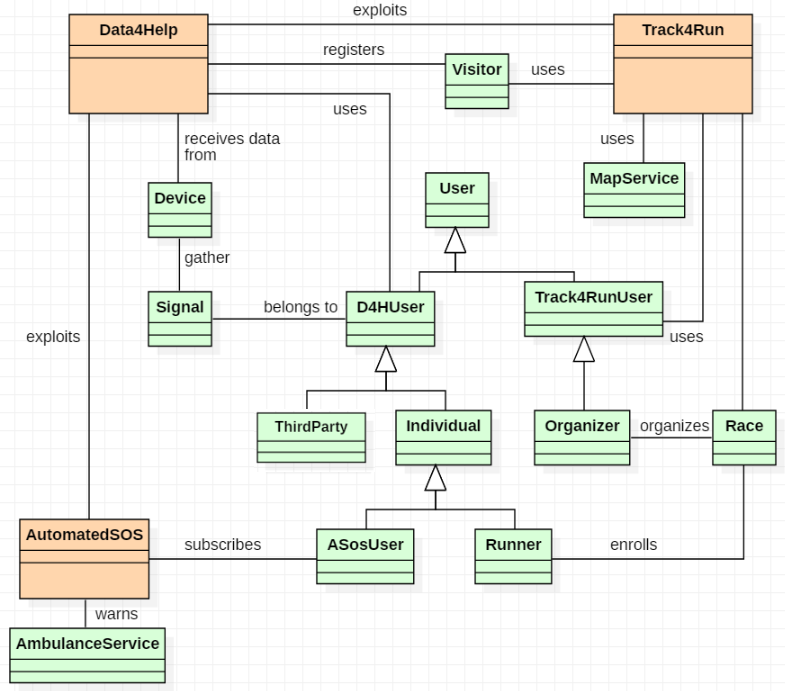
\includegraphics[scale=0.7]{./pictures/ClassDiagram.png}}%
    \caption{ Class diagram of the entire system}
    \label{fig:class-diagram}
\end{figure}

\section{Product functions}



\subsection{Data4Help }
[R] The system allows to third parties to request data of single users and to users to accept or refused them. 
    [R] If the user accepts, the system send to third party all the data gathered from the specified user.

    [R] If the user refused or he is not registered, the system sends to third party an error message.

[R] During registration, the system requires name, surname, fiscal code, password and email in order to create a new user account.

[R] During registration, the system requires the company name, partita IVA, email and password in order to create a new third party account.

[R] Upon third parties request, the system can perform parametric searches based on geographical areas, age, genre, time of the day. The result of the query is then stored and evaluated for approval.
    [R] If the request is approved, the saved data is provided to third party.
    [R] if the request is not approved, an error message is sent to the third party.
    [R] In order to anonimize data, the application only sends information related to the health status of individuals (e.g. bpm, step).
[R] The system allows to users to check gathered data.
[R] The system allows to third parties to access to their request history and results.

[R] The application allows third parties to subscribe to certain date
    [R] The application, if third party subscribed to some data (specific users or group searches), sends updates to the third party aggregating the data with the specified granularity and frequency.

[R] The application retrieves from smartwatches the following data, associating them to the user: 
\begin{itemize}
    \item beats per minute ( bpm );
    \item number of steps
    \item location
    \item timestamp of the measurement
\end{itemize}

[R] The application allows withdrawals of consent for accessing their data and third party unsubscriptions.
    [R] If the user withdraws consent for the access of his data, a message is sent to the subscribed third party and data is no longer provided.
    [R] If the third party no longer wishes to collect data from a specific user, a message is sent to him and his datais no longer sent.



\subsection{AutomatedSOS }

[R] The system has to analyse user date and sends the location of the user to the ambulance service in case of emergency, when health values goes under the threshold.

[R] The system gives the possibility to subscribe to the service upon request, only after checking the user age.

\subsection{Track4Run }

[R] the system allows participants to enrol just with their Data4Help account.

[R] The system allows the enrolling of runner only if they are not enrolled in a race at the same time.

[R] The system allows spectators to access the application as host-users, without registration, by giving them only the possibility to track the runners.

[R] The system store the ranks of old races so that both participants and organisers can access to the race history.

[R] The system should allow the registration of organisers without requiring also Data4Help registration,

[R] In order to organise a run, the application requires track, data, time and the maximum number of participants.

[R] The system need to update subscription to the runs, decreasing the number of allowed participants. It should not allow subscription if there are not leftovers places.

[R] The system shouldn't allow that two or more runs are organised neither at the same place and at the same time.

\section{User characteristics}
% here we include anything that is relevant to clarify their needs



\section{Assumption, dependencies and constraints}
% here we include domain assumptions

